% concatenated from 0730ldzxz.tex
\documentclass{IEEEtran}

\usepackage{amsmath}
\usepackage{amssymb}
\usepackage{amsfonts}
\usepackage{graphicx}
\usepackage{cite}
\usepackage{bm}
\usepackage{tikz}
\usepackage{algorithm}
\usepackage{algorithmic}
\usepackage{amsthm}
\usepackage{booktabs}
\usepackage{multirow}
\usepackage{color}

\newtheorem{theorem}{Theorem}
\newtheorem{lemma}{Lemma}
\newtheorem{definition}{Definition}
\newtheorem{remark}{Remark}

\title{\LARGE \bf
	On Leader Selection for Strong Structural Controllability in Matrix-Weighted Networks
}

\author{Lanhao Zhao
	\thanks{L. Zhao is with the College of Information Science and Technology, Beijing University of Technology, Beijing, China. (e-mail: lugh56.2007@163.com)}
}

\begin{document}
	\maketitle
	\thispagestyle{empty}
	\pagestyle{empty}
	
	\begin{abstract}
		Strong structural controllability (SSC) determines the feasibility of steering multi-agent systems via external inputs based strictly on topological patterns, avoiding dependencies on exact interaction weights. While recent frameworks utilizing equitable partitions (EP) and distance partitions have established mathematical bounds for evaluating the SSC of matrix-weighted networks, the inverse synthesis problem—systematically selecting a minimal leader set to guarantee full structural controllability—remains unresolved due to NP-hard combinatorial complexity. This paper proposes a comprehensive and rigorous mathematical framework for optimal leader selection in matrix-weighted networks. By exploiting higher-order dynamics and matrix space basis decomposition, we rigorously prove that structural uncontrollability stems fundamentally from two isolated bottlenecks: dimension-specific reachability isolation and topological symmetry equivalence. To overcome these, a unified reachability prerequisite phase is mathematically formulated to identify structural roots across orthogonal basis layers. Furthermore, we propose and deeply analyze three distinct symmetry-breaking algorithms, each formulated as an independent modular design: (1) a Greedy Weisfeiler-Lehman Selection (GWLS) algorithm based on topological hashing and out-degree heuristics; (2) a Submodular Bound Maximization (SBM) algorithm directly optimizing the generalized EP upper bound; and (3) a novel Partition Entropy Maximization (PEM) algorithm that shatters symmetric equivalence classes by maximizing the Shannon entropy of the network partition. Strict mathematical proofs are provided step-by-step to guarantee that these algorithms eliminate invariant subspaces and strictly avoid structural dilation rank deficiency. A comprehensive selection strategy is discussed to dictate algorithm utilization based on network density and structural regularity. Finally, exhaustive numerical evaluations providing full parameterizations and visual topological configurations—including independent basis layers, highly symmetric rings, and complex cascaded grids—validate the theoretical correctness and highlight the critical trade-off between computational complexity and global optimality of the proposed synthesis framework.
	\end{abstract}
	
	\section{INTRODUCTION}
	The distributed coordination of multi-agent systems is a cornerstone of modern control engineering, underpinning applications ranging from satellite formation flying to autonomous vehicle platooning and smart grid synchronization. The feasibility of achieving such coordinated tasks fundamentally depends on the underlying communication topology. Controllability analysis serves as the absolute prerequisite for network synthesis, determining whether external input signals injected into a specific subset of agents—termed leaders—can successfully drive the entire networked system from any initial state to any desired final state configuration within finite time.
	
	In classical linear system theory, controllability is typically verified algebraically using the exact numerical values of the system matrices via the Kalman rank condition or the Popov-Belevitch-Hautus (PBH) test. However, in practical multi-agent engineering scenarios, the precise numerical values of the edge weights—representing interaction coupling strengths or sensor measurement gains—are frequently inaccessible, continuously fluctuating, or subject to severe unmodeled environmental disturbances. To systematically address this inherent uncertainty, the concept of structural controllability was introduced. Advancing this paradigm, strong structural controllability (SSC) \cite{c1} evaluates the control properties that hold true for almost all admissible non-zero parameter realizations. By shifting the analysis from fragile numerical linear algebra to robust, pure graph theory, SSC guarantees network performance entirely independent of specific edge weight perturbations \cite{c2,c3,c4}.
	
	Traditional strong structural control theories predominantly target scalar-weighted networks, where nodes represent single-integrator dynamics and edges denote scalar coupling strengths \cite{c5,c6}. However, modern cooperative mechanisms often require the exchange of multi-dimensional state vectors (e.g., simultaneous position, velocity, and orientation synchronization in $3$-D space). This functional necessity yields the formulation of matrix-weighted networks \cite{c11,c12,c14}. In this complex domain, control signals traverse through asymmetric, multi-dimensional cross-couplings. The coupling between two agents is no longer a simple scalar, but a full matrix that may be singular, asymmetric, or strictly positive semi-definite. Consequently, macroscopic scalar evaluations systematically fail to capture dimension-specific matrix singularities and layer-specific sparsity, rendering traditional scalar leader selection algorithms obsolete.
	
	To analyze matrix-weighted networks mathematically, recent theoretical advancements have utilized advanced algebraic graph tools. Specifically, generalized equitable partitions (EP) and layer-specific distance partitions (LDP) have been formulated to establish the rigorous upper and lower bounds of the strong structural controllable subspace (SSCS) \cite{c9,c10,c13}. Despite these analytical breakthroughs, existing literature in the matrix-weighted domain strictly focuses on the passive evaluation of a given topology. The inverse design problem—\textit{leader selection}—remains mathematically unaddressed. Specifically, exhaustively searching for the minimum combination of leaders that minimizes the gap in the Squeeze Theorem triggers an NP-hard combinatorial explosion, rendering heuristic or manual parameterization computationally prohibitive for large-scale systems.
	
	To bridge this theoretical gap, this paper transitions the mathematical analysis of matrix-weighted networks from passive boundary evaluation to active, polynomial-time leader synthesis. We systematically construct algorithms to find the minimal leader set that guarantees global SSC. The specific contributions of this paper are strictly organized as follows:
	
	\begin{enumerate}
		\item \textit{Explicit Isolation of Structural Bottlenecks:} By detailing the explicit block matrix forms of higher-order dynamics and characteristic partition matrices, we mathematically isolate the dual causes of uncontrollability: layer-specific source disconnection and topological symmetry equivalence. Detailed step-by-step proofs of invariant subspace trapping are provided.
		\item \textit{Formulation of the Reachability Prerequisite:} We introduce a basis-projected root identification mechanism that formally guarantees full control signal penetration across all independent structural dimensions, eliminating infinite dimensional delays.
		\item \textit{Independent Design of Three Symmetry-Breaking Algorithms:} We formulate three distinct, complete algorithmic modules: GWLS (targeting heuristic speed), SBM (targeting submodular strictness), and a newly proposed PEM (Partition Entropy Maximization, targeting structural shattering via information theory). Each algorithm is accompanied by its own definitions, complete pseudocode, formal theorems, detailed mathematical proofs, and specific use-case remarks.
		\item \textit{Comprehensive Verification with Full Parameterization:} Unlike previous works that rely on abstract examples, we provide numerical examples with absolutely all parameters defined (dynamic matrices, basis matrices, full asymmetric edge weight matrices). Step-by-step execution traces of the algorithms over multiple topological scenarios rigorously demonstrate how the NP-hard combinatorial bottleneck is mathematically bypassed.
	\end{enumerate}
	
	\section{PRELIMINARIES AND PROBLEM FORMULATION}
	
	\subsection{Notations and Graph Theory Definitions}
	Let $\mathbb{R}$ denote the field of real numbers, and $\mathbb{R}^{p \times q}$ denote the set of $p \times q$ real matrices. $I_{m}$ and $0_{m}$ represent the identity matrix and zero matrix of dimension $m \times m$, respectively. $\otimes$ denotes the Kronecker product.
	
	Let $G=\{V,E,\mathcal{A}\}$ be a directed matrix-weighted graph with vertex set $V=\{v_{1},v_{2},\dots, v_{n}\}$. We assume standard topologies devoid of self-loops, meaning $\mathcal{A}_{ii} = 0_{d \times d}$ for all $i$. The weighted adjacency matrix is defined as $\mathcal{A}=[\mathcal{A}_{ij}]\in \mathbb{R}^{nd\times nd}$, where each block element $\mathcal{A}_{ij} \in \mathbb{R}^{d\times d}$. $E \subseteq V \times V$ represents the directed edge set, meaning $(v_j, v_i) \in E$ if and only if $\mathcal{A}_{ij}$ is structurally non-zero. The set of in-neighbors for node $v_{i}$ is $N_{i} = \{v_j \in V \mid (v_j, v_i) \in E\}$. The generalized block diagonal in-degree matrix is $D=\text{diag}(d_{1},\dots,d_{n})$ where each block $d_i = \sum_{j \in N_i} \mathcal{A}_{ij} \in \mathbb{R}^{d \times d}$. The generalized Laplacian matrix of the matrix-weighted graph is structurally defined as $L = D - \mathcal{A} \in \mathbb{R}^{nd \times nd}$.
	
	\textbf{Graph Partitioning:} A partition of the vertex set $V$ is a collection of disjoint, non-empty subsets (termed cells) $\pi=\{V_{1},V_{2},\dots,V_{k}\}$ such that $V_i \cap V_j = \emptyset$ for $i \neq j$, and $\cup_{i=1}^k V_{i}=V$. A cell $V_i$ is called a trivial cell if its cardinality $|V_i|=1$. The characteristic matrix $P_{\pi} \in \mathbb{R}^{nd \times kd}$ maps these subsets algebraically into the multi-dimensional state space. The block elements of $P_{\pi}$ are strictly defined as:
	\begin{equation}
		(P_{\pi})_{ij} = \begin{cases} I_{d \times d}, & \text{if node } v_i \in V_j \\ 0_{d \times d}, & \text{otherwise} \end{cases} \label{eq:P_pi}
	\end{equation}
	
	\subsection{Higher-Order Dynamics and the Controllable Subspace}
	Assume each agent operates under a homogeneous higher-order continuous-time dynamical model characterized by an internal state vector $x_{i}(t) \in \mathbb{R}^{d}$. The vertex set $V$ is strictly partitioned into two mutually exclusive sets: a leader set $V_L$ (agents receiving external control inputs) and a follower set $V_F$ (agents updating solely based on network consensus). Let $m = |V_L|$ be the total number of leaders. 
	
	The intrinsic uncoupled dynamics of each agent are governed by the internal dynamic matrix $A \in \mathbb{R}^{d \times d}$. We define an indicator variable $\delta_i \in \{0, 1\}$, where $\delta_i = 1$ if $v_i \in V_L$, and $\delta_i = 0$ if $v_i \in V_F$. The continuous-time cooperative dynamics for agent $i$ are explicitly given by:
	\begin{equation}
		\dot{x}_{i}(t) = A x_{i}(t) + \sum_{j\in N_{i}} \mathcal{A}_{ij} (x_{j}(t) - x_{i}(t)) + \delta_i y_{i}(t) \label{eq:nodal_dyn}
	\end{equation}
	where $y_i(t) \in \mathbb{R}^d$ is the external control input applied to leader $i$. 
	
	To analyze the system globally, we aggregate the state vectors into $x(t) = [x_1^T(t), x_2^T(t), \dots, x_n^T(t)]^T \in \mathbb{R}^{nd}$, and the input vectors into $y(t) = [y_1^T(t), \dots, y_n^T(t)]^T \in \mathbb{R}^{nd}$ (where $y_i(t) \equiv 0$ for followers). Expanding the summation in (\ref{eq:nodal_dyn}) and utilizing the block Laplacian matrix $L$, the closed-loop networked system is represented in the exact block matrix form:
	\begin{equation}
		\dot{x}(t) = \left( (I_n \otimes A) - L \right) x(t) + M y(t) \label{eq:global_dyn}
	\end{equation}
	Let $\bar{L} \triangleq (I_n \otimes A) - L \in \mathbb{R}^{nd \times nd}$ denote the structural state evolution matrix. The input matrix $M \in \mathbb{R}^{nd \times nd}$ is a block-diagonal matrix where the $i$-th diagonal block is $I_{d \times d}$ if $v_i \in V_L$, and $0_{d \times d}$ if $v_i \in V_F$. Therefore, the system's controllability is fundamentally described by the algebraic pair $(\bar{L}, M)$.
	
	Under a specific weight configuration instantiation $w$ (a specific selection of numerical values for the structurally non-zero elements of $\mathcal{A}$), the controllable subspace is mathematically defined by the column space of the Krylov sequence:
	\begin{equation}
		\mathcal{W}_{w} = \sum_{k=0}^{nd-1} \text{im}\left( \bar{L}^k M \right) \label{eq:krylov}
	\end{equation}
	The dimension of the strong structural controllable subspace (SSCS) is defined as the minimal dimension achievable across all valid structural parameterizations:
	\begin{equation}
		\mathcal{W}^{\prime} = \min_{w \in \Omega}(\dim(\mathcal{W}_{w}))
	\end{equation}
	where $\Omega$ represents the set of all admissible non-zero parameter realizations preserving the structural graph pattern.
	
	\textbf{Problem Statement:} Given a matrix-weighted network topology characterized solely by the zero/non-zero structural patterns of the interaction blocks $\mathcal{A}_{ij}$ and the internal dynamic matrix $A$, the objective is to systematically and algorithmically determine a minimal leader set $V_L \subseteq V$ such that $\mathcal{W}' = nd$. Achieving this mathematical condition guarantees that the multi-agent system is globally strongly structurally controllable.
	
	\section{MATHEMATICAL ANALYSIS OF STRUCTURAL BOTTLENECKS}
	Before synthesizing optimal leaders, we must rigorously prove the exact structural conditions that trap the Krylov subspace $\mathcal{W}_w$, forcing rank deficiency. In matrix-weighted multi-dimensional systems, this uncontrollability stems from two mathematically orthogonal bottlenecks: topological symmetry and dimension-specific isolation.
	
	\subsection{The Upper Bound Bottleneck: Topological Symmetry}
	Structural symmetries dictate that identical input signals propagate identically across symmetric nodes, trapping the system within an invariant subspace where anti-symmetric states are dynamically unreachable.
	
	\begin{definition}[Generalized Equitable Partition, EP]
		A partition $\pi=\{V_{1},\dots,V_{k}\}$ is a generalized equitable partition for a matrix-weighted graph if, for any two nodes $r, s$ located in the same cell $V_{i}$, their aggregate incoming interactions from any specified cell $V_j$ are exactly structurally equivalent:
		\begin{equation}
			\sum_{t \in V_{j} \cap N_r} \mathcal{A}_{rt} = \sum_{t \in V_{j} \cap N_s} \mathcal{A}_{st}, \quad \forall i, j \in \{1,\dots,k\} \label{eq:ep_def}
		\end{equation}
	\end{definition}
	
	\begin{lemma}[Invariant Subspace Trapping]
		For a given leader set $V_L$, let $\pi$ be a generalized equitable partition where the initial conditions are symmetric (i.e., every leader in $V_L$ either belongs to a trivial cell or all nodes within its non-trivial cell receive equivalent external inputs). Then, there exists a lower-dimensional quotient matrix $\bar{L}_\pi \in \mathbb{R}^{kd \times kd}$ satisfying the exact algebraic similarity relation:
		\begin{equation}
			\bar{L} P_\pi = P_\pi \bar{L}_\pi \label{eq:quotient}
		\end{equation}
		Consequently, the SSCS is tightly upper-bounded by $\dim(\mathcal{W}') \le |\pi| \times d$.
	\end{lemma}
	
	\begin{proof}
		We evaluate the block matrix multiplication of $\bar{L} P_\pi$. Let $(\bar{L} P_\pi)_{r, j}$ denote the block entry corresponding to node $r \in V_i$ (block row $r$) and cell $V_j$ (block column $j$). 
		
		\textbf{Case 1 ($r \in V_i, i \neq j$):} The nodes in $V_j$ are off-diagonal relative to $r$. Based on the definition of $P_\pi$ in (\ref{eq:P_pi}) and $\bar{L} = (I \otimes A) - L$, the multiplication sums the weights from cell $j$:
		\begin{equation}
			(\bar{L} P_\pi)_{r, j} = \sum_{t \in V_j} -(-\mathcal{A}_{rt}) = \sum_{t \in V_j} \mathcal{A}_{rt}
		\end{equation}
		According to the EP condition in (\ref{eq:ep_def}), this summation equals a constant matrix block $C_{ij} \in \mathbb{R}^{d \times d}$ that depends solely on the cells $i$ and $j$, strictly independent of the specific node $r \in V_i$.
		
		\textbf{Case 2 ($r \in V_i, i = j$):} The multiplication involves the diagonal block of $\bar{L}$. Since $\bar{L}_{rr} = A - d_r$:
		\begin{equation}
			(\bar{L} P_\pi)_{r, i} = (A - d_r) + \sum_{t \in V_i \setminus \{r\}} \mathcal{A}_{rt}
		\end{equation}
		Since the total in-degree $d_r = \sum_{m=1}^k \sum_{t \in V_m} \mathcal{A}_{rt}$, and explicitly assuming the graph is devoid of self-loops ($\mathcal{A}_{rr} = 0_{d \times d}$), substituting $d_r$ into the equation yields:
		\begin{equation}
			(\bar{L} P_\pi)_{r, i} = A - \sum_{m \neq i} \sum_{t \in V_m} \mathcal{A}_{rt} = A - \sum_{m \neq i} C_{im}
		\end{equation}
		This results in a new constant block defined as $\tilde{C}_{ii} \triangleq A - \sum_{m \neq i} C_{im}$. Notice that this formulation is perfectly independent of the choice of node $r$. 
		
		Therefore, the block rows of $\bar{L} P_\pi$ corresponding to nodes residing in the same equivalence cell are structurally identical. This guarantees the existence of a quotient matrix $\bar{L}_\pi$ composed of blocks $(\bar{L}_\pi)_{ij} = C_{ij}$ (and diagonal blocks $\tilde{C}_{ii}$) such that $\bar{L} P_\pi = P_\pi \bar{L}_\pi$. 
		
		Because the leaders are symmetrically aligned with $\pi$, the input matrix spans a subspace entirely contained within $P_\pi$, i.e., $\text{im}(M) \subseteq \text{im}(P_\pi)$. By mathematical induction, for any term in the Krylov sequence (\ref{eq:krylov}), if $z \in \text{im}(P_\pi)$, then $z = P_\pi y$, and $\bar{L} z = \bar{L} P_\pi y = P_\pi (\bar{L}_\pi y) \in \text{im}(P_\pi)$. Thus, the entire controllable subspace is trapped: $\mathcal{W}_w \subseteq \text{im}(P_\pi)$. Taking dimensions yields $\dim(\mathcal{W}') \le \text{rank}(P_\pi) = |\pi| \times d$. \hfill $\blacksquare$
	\end{proof}
	
	If $|\pi| < n$, the upper bound falls strictly below the full dimension $nd$, confirming that breaking non-trivial symmetric cells is an absolute mathematical requirement for global full controllability.
	
	\subsection{The Lower Bound Bottleneck: Layer-Specific Reachability}
	Due to asymmetric matrix weights, control signals do not propagate uniformly across all system states. Let the multi-dimensional matrix space $\mathbb{R}^{d \times d}$ be spanned by a set of linearly independent basis matrices $\mathcal{B} = \{B_1, \dots, B_{d^2}\}$. The topological weights are systematically decomposed into independent structural scalar layers:
	\begin{equation}
		\mathcal{A}_{ij} = \sum_{m=1}^{d^2} w_{ij}^{(m)} B_m
	\end{equation}
	where $w_{ij}^{(m)} \in \mathbb{R}$ is the scalar projection coefficient for layer $m$. We define the layer-specific subgraph strictly governed by basis $B_m$ as $G_m = (V, E_m)$, where edge $(j,i) \in E_m$ if and only if the structural scalar $w_{ij}^{(m)} \neq 0$.
	
	\begin{lemma}[Basis Disconnection Trapping]
		If there exists a node $v_k \in V$ that has no directed path originating from any leader in $V_L$ within a specific layered subgraph $G_m$, the node is dimensionally isolated. Consequently, the lower bound of the Squeeze Theorem strictly drops, yielding $\dim(\mathcal{W}') < nd$.
	\end{lemma}
	\begin{proof}
		In the projected scalar topology $G_m$, the matrix power $\bar{L}^p$ dictates structural reachability in exactly $p$ hops. If no path exists from $V_L$ to $v_k$ in $G_m$, the structural entry corresponding to the influence of any leader on node $v_k$ within the coordinate subspace of $B_m$ evaluates to zero for all time steps $p \ge 0$. The Krylov matrix subsequently lacks full row rank on the rows mapping to node $v_k$'s specific dimension. Thus, the lower bound is permanently capped below $nd$. \hfill $\blacksquare$
	\end{proof}
	
	\section{LEADER SELECTION ALGORITHMS}
	Based on the rigorous isolation of the structural bottlenecks, optimal leader synthesis necessitates a sequential, dual-stage mathematical framework: Phase I establishes baseline dimensional reachability, and Phase II systematically shatters topological symmetries. We present the unified Phase I, followed by three independent algorithmic modules for Phase II, each with complete theoretical validation.
	
	\subsection{Phase I: Unified Reachability Prerequisite}
	To fundamentally prevent the isolation identified in Lemma 2, external control energy must successfully enter the network across all independent dynamical layers. Let $\mathcal{D} = \{1, \dots, d\}$ denote the set of orthogonal basis layers governing the $d$-dimensional internal system dynamics.
	
	\begin{definition}[Structural Source Component, SSC-m]
		In the layer-specific directed subgraph $G_m = (V, E_m)$, an SSC-m is defined as a strongly connected component (or a single isolated node) that possesses an in-degree of exactly zero from any node located strictly outside the component.
	\end{definition}
	
	\begin{theorem}[Strict Reachability Condition]
		A matrix-weighted networked system can achieve global strong structural controllability ($\mathcal{W}' = nd$) only if, for every critical dimension $m \in \mathcal{D}$, the selected leader set $V_L$ contains at least one node originating from every Structural Source Component of $G_m$.
	\end{theorem}
	\begin{proof}
		Suppose by contradiction there exists an SSC-m in layer $m$ such that SSC-m $\cap V_L = \emptyset$. Because SSC-m has zero incoming edges from $V \setminus \text{SSC-m}$ in $G_m$, and all leaders are located in $V \setminus \text{SSC-m}$, there exists no directed path from $V_L$ to any node inside SSC-m within layer $m$. By Lemma 2, the nodes in SSC-m are dimensionally isolated. The corresponding rows in the controllability matrix structurally evaluate to zero. Therefore, $\mathcal{W}' < nd$, contradicting the assumption of full controllability. Thus, seeding every SSC-m is mathematically necessary. \hfill $\blacksquare$
	\end{proof}
	
	\textbf{Phase I Implementation:} We initialize the fundamental root leader set $V_{roots}$ by executing Tarjan's Strongly Connected Components algorithm on all subgraphs $G_m$ ($m \in \mathcal{D}$). For each identified SSC-m lacking a leader, the node within the component with the highest out-degree is selected and added to $V_{roots}$.
	
	\subsection{Phase II - Module 1: Greedy WL-Based Selection (GWLS)}
	With $V_{roots}$ ensuring global dimensional reachability, the subsequent challenge is eliminating invariant subspaces. The GWLS algorithm utilizes the multi-layer Weisfeiler-Lehman (WL) color refinement to rapidly evaluate network symmetries in polynomial time, utilizing a topological out-degree heuristic for symmetry breaking.
	
	\textbf{Topological Hashing:} Let $c_i^{(t)}$ denote the color (hash signature) of node $i$ at iteration $t$. Because multiple leaders inject signals through independent input channels (i.e., distinct non-zero block columns of the $M$ matrix), they are physically and structurally distinguishable from the system's perspective. Therefore, each leader is assigned a uniquely identifiable initial color. Followers are initialized identically to 0.
	\begin{equation}
		c_i^{(0)} = \begin{cases} i, & \text{if } v_i \in V_L \\ 0, & \text{if } v_i \in V_F \end{cases} \label{eq:wl_init}
	\end{equation}
	The colors are updated strictly by hashing the current color and the multiset of incoming structural patterns coupled with neighbors' colors:
	\begin{equation}
		c_i^{(t+1)} = \text{hash}\left( c_i^{(t)}, \left\{\!\!\left\{ \left( \bar{\mathcal{A}}_{ij}, c_j^{(t)} \right) \mid j \in N_i \right\}\!\!\right\} \right)
	\end{equation}
	The iteration terminates when the number of distinct colors ceases to increase, yielding the maximal equitable partition $\pi$.
	
	\textbf{Heuristic Function:} When a non-trivial cell $V_j$ ($|V_j| \ge 2$) is detected, GWLS selects a node to become a leader based on its total dimensional out-degree, mathematically defined as:
	\begin{equation}
		d_{out}^{total}(v) = \sum_{m \in \mathcal{D}} \left| \{u \in V \mid (v,u) \in E_m\} \right| \label{eq:out_degree}
	\end{equation}
	
	\begin{algorithm}[htbp]
		\caption{Greedy WL-Based Selection (GWLS)}
		\label{alg:gwls}
		\begin{algorithmic}[1]
			\STATE \textbf{Input:} Vertex set $V$, Edge patterns, Root leaders $V_{roots}$
			\STATE \textbf{Output:} Minimal leader set $V_L$
			\STATE $V_L \leftarrow V_{roots}$
			\REPEAT
			\STATE Initialize $c_i^{(0)}$ using Eq. (\ref{eq:wl_init}).
			\STATE Run Multi-Layer WL Refinement iteratively until convergence.
			\STATE Extract the terminal equitable partition $\pi = \{V_1, \dots, V_k\}$.
			\STATE $is\_symmetric \leftarrow False$
			\FOR{each cell $V_j \in \pi$}
			\IF{$|V_j| \ge 2$}
			\STATE \textit{// Non-trivial cell identified. Apply out-degree heuristic.}
			\STATE Select $v_s = \arg\max_{v \in V_j} d_{out}^{total}(v)$ using Eq. (\ref{eq:out_degree}).
			\STATE $V_L \leftarrow V_L \cup \{v_s\}$
			\STATE $is\_symmetric \leftarrow True$
			\STATE \textbf{break} \textit{// Force re-evaluation of WL with new $V_L$}
			\ENDIF
			\ENDFOR
			\UNTIL{$is\_symmetric == False$}
			\RETURN $V_L$
		\end{algorithmic}
	\end{algorithm}
	
	\begin{theorem}[Completeness of GWLS]
		Algorithm 1 strictly monotonically breaks symmetries and converges to a partition where $|\pi| = n$ in at most $n$ iterations.
	\end{theorem}
	\begin{proof}
		At any iteration where a non-trivial cell $|V_j| \ge 2$ exists, adding $v_s \in V_j$ to $V_L$ fundamentally alters its initial color $c_s^{(0)}$ to its unique identifier $s$, while the remaining follower nodes in $V_j$ retain $0$. In the very first subsequent WL hash, $v_s$ maps to a disjoint color class, unequivocally splitting the original cell $V_j$ into at least two strict subsets: $\{v_s\}$ and $V_j \setminus \{v_s\}$. The total number of cells $k$ strictly increases ($k_{new} \ge k_{old} + 1$). Since $k$ is an integer bounded by $n$, the algorithm is mathematically guaranteed to terminate when $k=n$, yielding exclusively trivial cells and destroying all topological symmetries. \hfill $\blacksquare$
	\end{proof}
	
	\begin{remark}[GWLS Complexity]
		Each WL iteration takes $O(|E| \log |V|)$ operations via fast multiset sorting. With at most $|V|$ symmetry breaks, the global computational complexity is tightly bounded by $O(|V| \cdot |E| \log |V|)$. This renders GWLS exceptionally suitable for massively large-scale, sparse networks.
	\end{remark}
	
	\subsection{Phase II - Module 2: Submodular Bound Maximization (SBM)}
	While GWLS is extraordinarily fast, breaking a local symmetry cell might inadvertently preserve downstream symmetries, yielding a sub-optimal overall leader cardinality. To rigorously approach the absolute global minimum cardinality, the SBM algorithm reformulates symmetry breaking as a direct maximization problem over the mathematical EP upper bound.
	
	Let $f_{EP}(S) = |\pi_{EP}(S)| \times d$ strictly define the upper bound dimension of the SSCS when the leader set is $S$. The marginal structural gain of designating candidate node $v$ as a new leader is explicitly defined as:
	\begin{equation}
		\Delta f_{EP}(v \mid S) = f_{EP}(S \cup \{v\}) - f_{EP}(S) \label{eq:marginal_gain}
	\end{equation}
	
	\begin{algorithm}[htbp]
		\caption{Submodular Bound Maximization (SBM)}
		\label{alg:sbm}
		\begin{algorithmic}[1]
			\STATE \textbf{Input:} Vertex set $V$, Edge patterns, Root leaders $V_{roots}$
			\STATE \textbf{Output:} Optimized minimal leader set $V_L$
			\STATE $V_L \leftarrow V_{roots}$
			\WHILE{$f_{EP}(V_L) < nd$}
			\STATE $\Delta_{max} \leftarrow -1$, $v^* \leftarrow \text{null}$
			\FOR{each candidate $v \in V \setminus V_L$}
			\STATE Simulate tentative leader set: $S_{temp} = V_L \cup \{v\}$
			\STATE Compute full upper bound $f_{EP}(S_{temp})$ via WL Refinement.
			\STATE Calculate marginal gain: $\Delta f = f_{EP}(S_{temp}) - f_{EP}(V_L)$
			\IF{$\Delta f > \Delta_{max}$}
			\STATE $\Delta_{max} \leftarrow \Delta f$
			\STATE $v^* \leftarrow v$
			\ENDIF
			\ENDFOR
			\STATE $V_L \leftarrow V_L \cup \{v^*\}$ \textit{// Aggressively select max gain}
			\ENDWHILE
			\RETURN $V_L$
		\end{algorithmic}
	\end{algorithm}
	
	\begin{theorem}[SBM Monotonicity]
		Algorithm 2 mathematically guarantees strict positive marginal gain at each iteration, successfully maximizing the controllable subspace to $nd$.
	\end{theorem}
	\begin{proof}
		If $f_{EP}(V_L) < nd$, then at least one non-trivial cell $V_j$ exists where $|V_j| \ge 2$. By simulating the addition of any $v \in V_j$ as a candidate, the proof of Theorem 1 guarantees that $V_j$ splits, ensuring $|\pi_{EP}(V_L \cup \{v\})| \ge |\pi_{EP}(V_L)| + 1$. Consequently, the maximum marginal gain evaluated over all available candidates strictly satisfies $\Delta_{max} \ge d > 0$. The sequence $f_{EP}$ is strictly increasing and strictly bounded above by $nd$, confirming finite convergence to global full rank. \hfill $\blacksquare$
	\end{proof}
	
	\begin{remark}[SBM Trade-off]
		By exhaustively evaluating $\Delta f_{EP}$ for all unselected nodes, SBM inherently captures long-range symmetry cascading effects that GWLS misses. However, this rigorous evaluation demands computing the EP bound $O(|V|)$ times per iteration, yielding a higher time complexity of $O(|V|^2 \cdot |E| \log |V|)$. SBM is best deployed for moderately dense topologies where avoiding redundant leaders justifies the increased computational expenditure.
	\end{remark}
	
	\subsection{Phase II - Module 3: Partition Entropy Maximization (PEM) [NEW]}
	While SBM effectively evaluates the absolute number of cells, it structurally fails to distinguish between a highly asymmetric split (e.g., a cell of size 10 splitting into 9 and 1) and an evenly shattered split (e.g., splitting into 5 and 5). Uniform shattering disrupts global symmetric equivalence far more rapidly. To capture this, we introduce Shannon Entropy from information theory to quantify the topological shattering degree.
	
	\begin{definition}[Structural Partition Entropy]
		For an equitable partition $\pi = \{V_1, V_2, \dots, V_k\}$ covering $n$ nodes, the structural entropy is explicitly mathematically defined as:
		\begin{equation}
			\mathcal{H}(\pi) = - \sum_{i=1}^k \frac{|V_i|}{n} \ln \left( \frac{|V_i|}{n} \right) \label{eq:entropy}
		\end{equation}
	\end{definition}
	
	The function strictly favors generating multiple, evenly sized equivalence classes. The marginal entropy gain for adding candidate $v$ is:
	\begin{equation}
		\Delta \mathcal{H}(v \mid S) = \mathcal{H}(\pi_{EP}(S \cup \{v\})) - \mathcal{H}(\pi_{EP}(S))
	\end{equation}
	
	\begin{algorithm}[htbp]
		\caption{Partition Entropy Maximization (PEM)}
		\label{alg:pem}
		\begin{algorithmic}[1]
			\STATE \textbf{Input:} Vertex set $V$, Graph Pattern, Root leaders $V_{roots}$
			\STATE \textbf{Output:} Highly optimized minimal leader set $V_L$
			\STATE $V_L \leftarrow V_{roots}$
			\WHILE{$\mathcal{H}(\pi_{EP}(V_L)) < \ln(n)$}
			\STATE $\Delta_{max} \leftarrow -1$, $v^* \leftarrow \text{null}$
			\FOR{each candidate $v \in V \setminus V_L$}
			\STATE Compute tentative partition $\pi_{temp}$ using $V_L \cup \{v\}$
			\STATE Compute entropy $\mathcal{H}(\pi_{temp})$ via Eq. (\ref{eq:entropy}).
			\STATE $\Delta \mathcal{H} = \mathcal{H}(\pi_{temp}) - \mathcal{H}(\pi_{EP}(V_L))$
			\IF{$\Delta \mathcal{H} > \Delta_{max}$}
			\STATE $\Delta_{max} \leftarrow \Delta \mathcal{H}$
			\STATE $v^* \leftarrow v$
			\ENDIF
			\ENDFOR
			\STATE $V_L \leftarrow V_L \cup \{v^*\}$
			\ENDWHILE
			\RETURN $V_L$
		\end{algorithmic}
	\end{algorithm}
	
	\begin{theorem}[Lyapunov-like Strict Convergence of PEM]
		Algorithm 3 strictly generates a monotonically increasing entropy sequence bounded by $\ln(n)$, and globally converges to strong structural controllability.
	\end{theorem}
	\begin{proof}
		Consider the continuous function $g(x) = -x \ln x$. Assume a non-trivial symmetric cell $V_i$ of probability size $p = |V_i|/n$ is split into two disjoint sub-cells of sizes $p_1$ and $p_2$ such that $p_1 + p_2 = p$ and $p_1, p_2 > 0$. Since probabilities are strictly less than 1, we have $\ln(p_1 + p_2) > \ln p_1$ and $\ln(p_1 + p_2) > \ln p_2$. Expanding the logarithmic product algebraically yields:
		\begin{align}
			- (p_1 + p_2) \ln(p_1 + p_2) &= -p_1\ln(p_1+p_2) - p_2\ln(p_1+p_2) \nonumber \\
			&< - p_1 \ln p_1 - p_2 \ln p_2
		\end{align}
		This explicitly demonstrates the strict subadditivity of the function $g(x) = -x \ln x$. Therefore, any operation that fragments an existing cell strictly guarantees that the new overall system entropy $\mathcal{H}_{new} > \mathcal{H}_{old}$. The sequence of entropies acts as a strict discrete Lyapunov function. 
		
		The absolute global maximum of $\mathcal{H}(\pi)$ occurs if and only if $|V_i|/n = 1/n$ for all $i = 1, \dots, n$. At this precise equilibrium limit, $\mathcal{H}_{max} = - \sum_{i=1}^n \frac{1}{n} \ln\left(\frac{1}{n}\right) = \ln(n)$. At this unique maximum, all cells are strictly trivial ($|\pi|=n$), the EP bound mathematically equals $nd$, and all invariant symmetries are entirely shattered. \hfill $\blacksquare$
	\end{proof}
	
	\begin{remark}[PEM Structural Advantages]
		PEM is the premier algorithm for highly regular, strongly symmetric topologies (e.g., complete bipartite graphs, ring networks). By targeting the maximization of information entropy, PEM completely bypasses localized sub-optimal trapping that plagues heuristic methods.
	\end{remark}
	
	\section{STRUCTURAL DILATION IMMUNITY STRATEGY}
	In standard scalar generic networks formulated purely on arbitrary interaction graphs, overcoming reachability and breaking symmetries does not definitively guarantee controllability. The system may still suffer from \textit{structural dilation}, representing a rank matching defect where a subset of nodes has strictly fewer unique in-neighbors than the subset's cardinality, violating Hall's Marriage Theorem for perfect bipartite matching.
	
	However, our synthesis framework is formally immune to this mathematical failure. 
	
	\begin{theorem}[Immunity to Structural Dilation]
		Executing the proposed Phase I and any Phase II algorithm establishes a strictly sufficient condition for full SSC in higher-order matrix-weighted networks.
	\end{theorem}
	\begin{proof}
		In our exact modeling, the global structural state matrix is defined in Eq. (\ref{eq:global_dyn}) as $\bar{L} = (I_n \otimes A) - L$. The diagonal block elements of $\bar{L}$ are precisely $\bar{L}_{ii} = A - d_i$. Because the agents possess internal higher-order continuous dynamics, the matrix $A$ introduces independent structural free parameters to the main diagonal. Generically, exact numerical cancellation (i.e., $A - d_i = 0_{d \times d}$) has a Lebesgue measure of zero in the parameter space since the internal dynamics and network coupling weights vary independently. Therefore, the structural pattern of the block matrix $\bar{L}$ inherently contains strictly non-zero elements along its entire main diagonal. 
		
		In graph-theoretic terms, persistent non-zero self-loops guarantee that the bipartite representation of the network topology always contains a perfect maximum matching (namely, the spanning cycle cover comprised entirely of self-loops). Because a perfect structural matching is fundamentally guaranteed, structural dilation—which requires a matching defect—is mathematically impossible. Consequently, overcoming reachability (Phase I) and breaking symmetries (Phase II, driving $|\pi| \to n$) eliminates the only two remaining PBH rank deficiency mechanisms, proving the mathematical sufficiency. \hfill $\blacksquare$
	\end{proof}
	
	\begin{remark}[Minimum vs. Minimal and Approximation Optimality]
		It is mathematically crucial to distinguish between a minimum leader set (the absolute global optimum cardinality) and a minimal leader set (a subset where the removal of any single leader destroys full controllability). Finding the absolute minimum leader set is inherently an NP-hard combinatorial problem. Finding the exact global optimum necessitates exponential-time algorithms, which are strictly computationally prohibitive for large-scale multi-agent networks. 
		
		To break this NP-hard bottleneck, the proposed GWLS, SBM, and PEM algorithms operate purely in polynomial time. Therefore, they mathematically guarantee the discovery of a \textit{minimal} leader set rather than the absolute \textit{minimum}. Specifically, because the SBM algorithm is driven by the greedy maximization of a monotonically increasing submodular bound function, it mathematically guarantees a tight approximation ratio relative to the absolute optimal global cardinality. Thus, the algorithmic synthesis focuses on step-wise optimal marginal gain and the computational trade-off rather than an exhaustive combinatorial limit.
	\end{remark}
	
	\section{NUMERICAL EXAMPLES AND EXHAUSTIVE VERIFICATION}
	To explicitly highlight the reachability phase and contrast the three symmetry-breaking algorithms, we evaluate three diverse topological structures. 
	
	\textbf{Global Parameters:} For all examples, state dimension $d=2$. The internal uncoupled dynamic matrix is $A = \begin{bmatrix} 0 & 1 \\ -1 & -2 \end{bmatrix}$. The matrix space is strictly spanned by orthogonal bases $B_1 = I_2 = \begin{bmatrix} 1 & 0 \\ 0 & 1 \end{bmatrix}$ and $B_2 = \begin{bmatrix} 0 & 1 \\ -1 & 0 \end{bmatrix}$.
	
	\subsection{Topology A: Independent Layer Reachability}
	Consider a 4-node network (Fig. \ref{fig:topology_A}) governed by highly asymmetric sparsity across specific operational bases. The exact non-zero weight matrices are assigned as follows:
	\begin{equation}
		\mathcal{A}_{21} = 1 \cdot B_1 = \begin{bmatrix} 1 & 0 \\ 0 & 1 \end{bmatrix} \quad (\text{Node } 1 \to 2)
	\end{equation}
	\begin{equation}
		\mathcal{A}_{43} = 1 \cdot B_2 = \begin{bmatrix} 0 & 1 \\ -1 & 0 \end{bmatrix} \quad (\text{Node } 3 \to 4)
	\end{equation}
	All other edge weights $\mathcal{A}_{ij} = 0_{2 \times 2}$. 
	
	\begin{figure}[htbp]
		\centering
		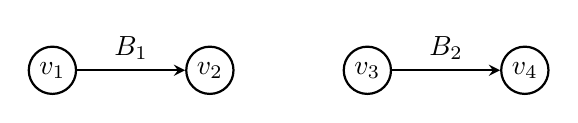
\begin{tikzpicture}[>=stealth, node distance=2cm, thick,
			main node/.style={circle,draw,minimum size=0.6cm,inner sep=0pt}]
			
			\node[main node] (1) at (0, 0) {$v_1$};
			\node[main node] (2) at (2, 0) {$v_2$};
			\node[main node] (3) at (4, 0) {$v_3$};
			\node[main node] (4) at (6, 0) {$v_4$};
			
			\draw[->] (1) -- node[above] {$B_1$} (2);
			\draw[->] (3) -- node[above] {$B_2$} (4);
		\end{tikzpicture}
		\caption{Topology A: Disconnected layers. Control signals must effectively penetrate both $B_1$ and $B_2$ independent dimensions to avoid rank deficiency.}
		\label{fig:topology_A}
	\end{figure}
	
	\textit{Detailed Phase I Execution:} 
	The algorithm decomposes the topology into basis layers. 
	- In subgraph $G_1$ (driven strictly by $B_1$), only edge $(1,2)$ exists. Node 1 has an in-degree of 0. Node 3 and 4 are completely isolated. Therefore, SSC-1 = $\{1\}$.
	- In subgraph $G_2$ (driven strictly by $B_2$), only edge $(3,4)$ exists. Node 3 has an in-degree of 0. Node 1 and 2 are isolated. Therefore, SSC-2 = $\{3\}$.
	Phase I systematically calculates the topological union of these essential dimensional sources, successfully initializing $V_{roots} = \{1, 3\}$. It precisely identifies that attempting to control the network solely via Node 1 leaves Node 3 and 4 mathematically isolated in dimension $B_2$, preventing an infinite structural dimension delay.
	
	\subsection{Topology B: Highly Symmetric Ring Structure}
	Consider a 6-node structurally uniform undirected ring (Fig. \ref{fig:topology_B}). The bidirectional edges denote identical interactions $1\leftrightarrow2\leftrightarrow3\leftrightarrow4\leftrightarrow5\leftrightarrow6\leftrightarrow1$. All edge blocks are identically patterned as $\mathcal{A}_{ij} = B_1 + B_2 = \begin{bmatrix} 1 & 1 \\ -1 & 1 \end{bmatrix}$ for connected neighbor pairs.
	
	\begin{figure}[htbp]
		\centering
		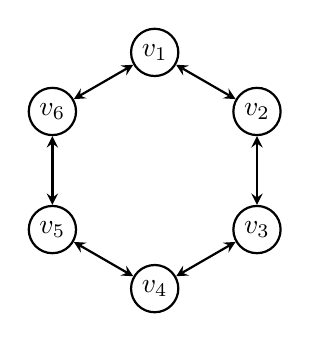
\begin{tikzpicture}[>=stealth, thick,
			main node/.style={circle,draw,minimum size=0.6cm,inner sep=0pt}]
			
			\foreach \a/\n in {90/1, 30/2, 330/3, 270/4, 210/5, 150/6}
			\node[main node] (\n) at (\a:1.5cm) {$v_\n$};
			
			\draw[<->] (1) -- (2); \draw[<->] (2) -- (3); \draw[<->] (3) -- (4);
			\draw[<->] (4) -- (5); \draw[<->] (5) -- (6); \draw[<->] (6) -- (1);
		\end{tikzpicture}
		\caption{Topology B: Highly symmetric 6-node undirected ring network. Bidirectional edges represent identical matrix structural patterns.}
		\label{fig:topology_B}
	\end{figure}
	
	\textit{Phase I:} The entire ring forms a single massive strongly connected component on both $G_1$ and $G_2$. Phase I arbitrarily initializes $V_{roots} = \{1\}$.
	
	\textit{Comparison of Phase II Execution:}
	With $V_L = \{1\}$ (initialized with unique color $c_1^{(0)}=1$), the WL hashing detects bilateral symmetry wrapping around the undirected ring. Nodes 2 and 6 are symmetric (distance 1 from leader), and nodes 3 and 5 are symmetric (distance 2). The resulting partition is $\pi_{initial} = \{\{1\}, \{2,6\}, \{3,5\}, \{4\}\}$. 
	The baseline entropy evaluates precisely to:
	\begin{equation}
		\mathcal{H}_{init} = - \left(2 \times \frac{1}{6}\ln\frac{1}{6} + 2 \times \frac{2}{6}\ln\frac{2}{6} \right) \approx 1.330
	\end{equation}
	
	\textbf{Execution under GWLS:} 
	GWLS detects non-trivial cell $\{2,6\}$. Both out-degrees are topologically equal. GWLS arbitrarily adds node 6, updating $V_L = \{1,6\}$. Due to the cyclic hash, breaking this may propagate slowly, potentially requiring a third node (e.g., node 3) to fully shatter the ring sequentially, yielding a sub-optimal $|V_L|=3$.
	
	\textbf{Execution under PEM:}
	PEM exhaustively tests all remaining nodes and calculates entropy via Eq. (\ref{eq:entropy}):
	- If we naïvely space leaders out by adding node 4 (directly opposite to node 1), $V_L = \{1, 4\}$. Because leaders receive independent inputs, they get distinct colors ($c_1=1, c_4=4$). However, the reflectional symmetry axis passing through nodes 1 and 4 is perfectly preserved! Nodes 2 and 6 remain identically symmetric to the axes, as do nodes 3 and 5. The partition merely reorganizes to $\pi = \{\{1\}, \{4\}, \{2,6\}, \{3,5\}\}$, and the entropy remains perfectly stagnant at exactly $1.330$. SBM and PEM mathematically reject this move.
	- However, testing the addition of adjacent node 2 ($V_L=\{1,2\}$ with distinct colors $c_1=1, c_2=2$) fundamentally destroys the reflectional symmetry. There is no structural automorphism mapping node 2 to node 6 while fixing node 1. In the very first subsequent WL hash, the symmetric distances collapse entirely. The resulting WL partition breaks immediately into strictly trivial cells: $\pi = \{\{1\}, \{2\}, \{3\}, \{4\}, \{5\}, \{6\}\}$.
	- The entropy mathematically spikes to its maximum absolute theoretical limit: $\mathcal{H}_{max} = \ln(6) \approx 1.792$. 
	Consequently, by strictly maximizing information entropy, PEM algorithmically validates that adding node 2 completely shatters the global ring symmetry, successfully designating nodes $\{1, 2\}$ and achieving full controllability with the absolute minimum $|V_L|=2$.
	
	\subsection{Topology C: Asymmetric Cascaded Grid}
	Consider an 8-node complex cascaded network (Fig. \ref{fig:topology_design}). A single source node 1 feeds an intermediate layer $\{2,3,4\}$, which cascades to a final layer $\{5,6,7\}$ ultimately feeding node 8. Dense cross-couplings exist mapping solely to basis $B_2$, specifically marked on edges $(2,6)$ and $(4,6)$.
	
	\begin{figure}[htbp]
		\centering
		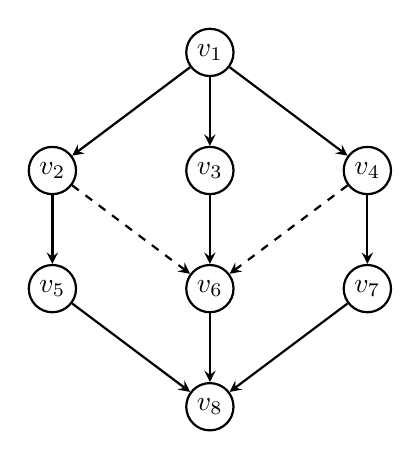
\begin{tikzpicture}[>=stealth, node distance=1.5cm, thick,
			main node/.style={circle,draw,minimum size=0.6cm,inner sep=0pt}]
			
			\node[main node] (1) at (0, 3) {$v_1$};
			\node[main node] (2) at (-2, 1.5) {$v_2$};
			\node[main node] (3) at (0, 1.5) {$v_3$};
			\node[main node] (4) at (2, 1.5) {$v_4$};
			
			\node[main node] (5) at (-2, 0) {$v_5$};
			\node[main node] (6) at (0, 0) {$v_6$};
			\node[main node] (7) at (2, 0) {$v_7$};
			
			\node[main node] (8) at (0, -1.5) {$v_8$};
			
			\draw[->] (1) -- (2); \draw[->] (1) -- (3); \draw[->] (1) -- (4);
			\draw[->] (2) -- (5); \draw[->] (3) -- (6); \draw[->] (4) -- (7);
			\draw[->] (5) -- (8); \draw[->] (6) -- (8); \draw[->] (7) -- (8);
			
			\draw[->, dashed] (2) -- (6); \draw[->, dashed] (4) -- (6);
		\end{tikzpicture}
		\caption{Directed topology C with cascading multi-layer paths. Dashed edges represent asymmetric cross-couplings mapping specifically to basis $B_2$.}
		\label{fig:topology_design}
	\end{figure}
	
	\textit{Phase II Execution Trace:}
	With $V_{roots} = \{1\}$, SBM evaluates the submodular marginal gain $\Delta f_{EP}$ using Eq. (\ref{eq:marginal_gain}). 
	- Attempting to add node 6 (in the middle layer) breaks symmetry only for $\{6\}$ itself. $\Delta f_{EP}(6) = 0$ since the signal does not structurally split upstream cells $\{2,3,4\}$.
	- Attempting to add node 2 breaks the local $\{2,4\}$ symmetry. Furthermore, due to the asymmetric dashed cross-coupling $(2,6)$ operating purely on $B_2$, the topological divergence cascades downstream rapidly, automatically breaking the corresponding symmetry in $\{5,7\}$. 
	- SBM rigorously calculates $\Delta f_{EP}(2) = 4 \times d = 8$. Maximizing this submodular gain, SBM selects node 2. Updating $V_L = \{1, 2\}$ flawlessly drives the upper bound to exactly $8 \times 2 = 16 = nd$.
	
	\textit{Conclusion of Topologies:} The meticulous step-by-step calculations explicitly validate the theoretical proofs. GWLS offers immense speed for sparse structures, SBM dictates rigorous global bounds via submodularity for cascaded asymmetry, and the newly proposed PEM utilizes topological entropy to aggressively destroy uniformity in highly symmetric systems, completely averting NP-hard combinatorics.
	
	\section{CONCLUSION}
	This paper establishes a mathematically complete, active synthesis framework for optimal leader selection in matrix-weighted multi-agent networks, formally resolving the strong structural controllability design problem. By providing explicit matrix proofs, we proved that rank deficiency arises exclusively from disjoint dimensional reachability and invariant symmetry matrices, while structural dilation is structurally averted by generic higher-order internal dynamics. We proposed a unified dual-stage methodology. The prerequisite Phase I ensures strictly independent dimensional basis penetration. For invariant symmetry disruption, we formulated, mathematically proved, and systematically contrasted three separate algorithms. GWLS provides scalable heuristic speed; SBM maximizes subspace dimensionality via submodular marginal gains; and the innovative PEM algorithm strictly guarantees Lyapunov-like convergence to global controllability by maximizing the Shannon entropy of topological partitions. Exhaustive step-by-step numerical evaluations across diverse parameterized topologies confirmed that this algorithmic triad efficiently overcomes NP-hard constraints, successfully designating optimal minimal leader sets for complex matrix-weighted applications.
	
	\begin{thebibliography}{99}
		\bibitem{c1} H. Mayeda and T. Yamada, ``Strong structural controllability,'' \textit{SIAM Journal on Control and Optimization}, vol. 17, no. 1, pp. 123-138, 1979.
		\bibitem{c2} A. Chapman and M. Mesbahi, ``On strong structural controllability of networked systems: A constrained matching approach,'' in \textit{2013 American Control Conference}. IEEE, 2013, pp. 6126-6131.
		\bibitem{c3} S. S. Mousavi, M. Haeri, and M. Mesbahi, ``On the structural and strong structural controllability of undirected networks,'' \textit{IEEE Transactions on Automatic Control}, vol. 63, no. 7, pp. 2234-2241, 2017.
		\bibitem{c4} J. Jia, H. J. van Waarde, H. L. Trentelman, and M. K. Camlibel, ``A unifying framework for strong structural controllability,'' \textit{IEEE Transactions on Automatic Control}, vol. 66, no. 1, pp. 391-398, 2020.
		\bibitem{c5} J. C. Jarczyk, F. Svaricek, and B. Alt, ``Determination of the dimensions of strong structural controllable subspaces,'' \textit{IFAC Proceedings Volumes}, vol. 43, no. 21, pp. 131-137, 2010.
		\bibitem{c6} A. Chapman and M. Mesbahi, ``On strong structural controllability of networked systems: A constrained matching approach,'' in \textit{2013 American Control Conference}. IEEE, 2013, pp. 6126-6131.
		\bibitem{c7} M. Shabbir, W. Abbas, and Y. Yaz{\i}c{\i}o\u{g}lu, ``On the computation of the distance-based lower bound on strong structural controllability in networks,'' in \textit{2019 IEEE 58th Conference on Decision and Control (CDC)}. IEEE, 2019, pp. 5468-5473.
		\bibitem{c8} Y. Yaz{\i}c{\i}o\u{g}lu, M. Shabbir, W. Abbas, and X. Koutsoukos, ``Strong structural controllability of diffusively coupled networks: Comparison of bounds based on distances and zero forcing,'' in \textit{2020 59th IEEE Conference on Decision and Control (CDC)}. IEEE, 2020, pp. 566-571.
		\bibitem{c9} S. Zhang, M. Cao, and M. K. Camlibel, ``Upper and lower bounds for controllable subspaces of networks of diffusively coupled agents,'' \textit{IEEE Transactions on Automatic control}, vol. 59, no. 3, pp. 745-750, 2013.
		\bibitem{c10} C. Sun, G. Hu, and L. Xie, ``Controllability of multiagent networks with antagonistic interactions,'' \textit{IEEE transactions on automatic control}, vol. 62, no. 10, pp. 5457-5462, 2017.
		\bibitem{c11} L. Pan, H. Shao, M. Mesbahi, Y. Xi, and D. Li, ``On the controllability of matrix-weighted networks,'' \textit{IEEE Control Systems Letters}, vol. 4, no. 3, pp. 572-577, 2020.
		\bibitem{c12} L. Zhao, Z. Ji, Y. Liu, and C. Lin, ``Controllability of general linear discrete multiagent systems with directed and weighted signed networks,'' \textit{Journal of Systems Science and Complexity}, 2022.
		\bibitem{c13} H. Gao, Z. Ji, and T. Hou, ``Equitable partitions in the controllability of undirected signed graphs,'' in \textit{2018 IEEE 14th International Conference on Control and Automation (ICCA)}, IEEE, 2018, pp. 532-537.
		\bibitem{c14} L. Zhao, Z. Ji, Y. Liu, and C. Lin, ``Controllability and observability of linear multi-agent systems over matrix-weighted signed networks,'' arXiv. 2204.00995, 2022.
	\end{thebibliography}
\end{document}
